\documentclass{beamer}
%
% Choose how your presentation looks.
%
% For more themes, color themes and font themes, see:
% http://deic.uab.es/~iblanes/beamer_gallery/index_by_theme.html
%
\mode<presentation>
{
  \usetheme{default}      % or try Darmstadt, Madrid, Warsaw, ...
  \usecolortheme{default} % or try albatross, beaver, crane, ...
  \usefonttheme{default}  % or try serif, structurebold, ...
  \setbeamertemplate{navigation symbols}{}
  \setbeamertemplate{caption}[numbered]
} 

\usepackage[english]{babel}
\usepackage[utf8]{inputenc}
\usepackage[T1]{fontenc}

\title[Your Short Title]{Projet de département  : Formation de patterns dans les systèmes de réaction-diffusion}
\author{Cyril NEDERVEEN\\
Louise HUREL\\
Audrey GOSSARD\\
Dana ZILBERBERG}
\institute{Ecole des Ponts Paristech}

\begin{document}

\begin{frame}
  \titlepage
\end{frame}

% Uncomment these lines for an automatically generated outline.
%\begin{frame}{Outline}
%  \tableofcontents
%\end{frame}

\section{Introduction}

\begin{frame}{Introduction}

\begin{itemize}
  \item Your introduction goes here!
  \item Use \texttt{itemize} to organize your main points.
\end{itemize}

\vskip 1cm

\begin{block}{Examples}
Some examples of commonly used commands and features are included, to help you get started.
\end{block}

\end{frame}

\section{Some \LaTeX{} Examples}

\subsection{Tables and Figures}

\begin{frame}{Tables and Figures}

\begin{itemize}
\item Use \texttt{tabular} for basic tables --- see Table~\ref{tab:widgets}, for example.
\item You can upload a figure (JPEG, PNG or PDF) using the files menu. 
\item To include it in your document, use the \texttt{includegraphics} command (see the comment below in the source code).
\end{itemize}

% Commands to include a figure:
%\begin{figure}
%\includegraphics[width=\textwidth]{your-figure's-file-name}
%\caption{\label{fig:your-figure}Caption goes here.}
%\end{figure}

\begin{table}
\centering
\begin{tabular}{l|r}
Item & Quantity \\\hline
Widgets & 42 \\
Gadgets & 13
\end{tabular}
\caption{\label{tab:widgets}An example table.}
\end{table}

\end{frame}

\subsection{Mathematics}

\begin{frame}{Readable Mathematics}

Let $X_1, X_2, \ldots, X_n$ be a sequence of independent and identically distributed random variables with $\text{E}[X_i] = \mu$ and $\text{Var}[X_i] = \sigma^2 < \infty$, and let
\[ S_n = \frac{X_1 + X_2 + \cdots + X_n}{n}
      = \frac{1}{n}\sum_{i}^{n} X_i \]
denote their mean. Then as $n$ approaches infinity, the random variables $\sqrt{n}(S_n - \mu)$ converge in distribution to a normal $\mathcal{N}(0, \sigma^2)$.

\end{frame}

\subsection{Résolution par la méthode d’Euler implicite}

\begin{frame}{Résolution par la méthode d’Euler implicite}
\textbf{Définition des variables et des paramètres :}
\begin{itemize}
    \item $a = 0.2$ et $b = 1.3$ (pour satisfaire $(a+b)^3>b-a$ et $b>a$.\\
    \item $N_x$ le nombre d'it\'erations sur la variable d'espace, $x \in [0;1]$\\
    \item $c = \begin{pmatrix} u \\ v \end{pmatrix}$, de taille $2 N_x$.\\
    \item $dt = 10^{-3}$ et $N_t = 50 000$
    \item variable $stock$ de taille $(2N_x,N_t)$ pour stocker toutes les concentrations
\end{itemize}

\end{frame}

\begin{frame}{Résolution par la méthode d’Euler implicite}
\textbf{Initialisation autour de la solution d'\'equilibre :}
aléatoirement autour de $u_{eq}$ et $v_{eq}$ à $10^{-4}$\\
\begin{figure}
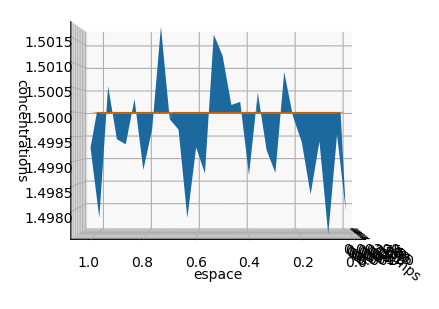
\includegraphics[width=\textwidth]{cond_init.png}
\caption{\label{fig:your-figure}Conditions initiales}
\end{figure}

\end{frame}

\begin{frame}{Résolution par la méthode d’Euler implicite}
\textbf{Equation du schéma}
à l'instant $t_n = n dt$\\
\begin{equation}
c^{n+1} = c^n + dt (DA c^{n+1} + \delta f(c^{n+1}))
\end{equation}
avec D = \begin{pmatrix} 
I  & 0 \\
 0  & dI
\end{pmatrix} et A = \begin{pmatrix} 
Lp  & 0 \\
 0  & Lp
\end{pmatrix}\\ où
\begin{displaymath}
Lp = \frac{1}{dx^2} \begin{pmatrix} 
-2     & 1     & 0      & \cdots & 1\\
 1     & -2    & \ddots & \ddots & \vdots\\
 0     &\ddots & \ddots & \ddots & 0\\
\vdots & \ddots& \ddots & \ddots & 1\\
1      &\cdots & 0      &    1   & -2
\end{pmatrix}
\end{displaymath}

\end{frame}

\begin{frame}{Résolution par la méthode d’Euler implicite}
\textbf{Simplification du schéma :}
\begin{align}
c^{n+1} = c^n + dt (DA c^{n+1} + \delta f(c^n)) \nonumber\\
\nonumber \\
c^{n+1} = (I - dt DA)^{-1} (c^n + dt \delta f(c^n))
\end{align}\\
\textbf{Stockage :}
\begin{equation}
stock(n, 1:2 N_x) = c^n
\end{equation}\\
\end{frame}

\begin{frame}{Résolution par la méthode d’Euler implicite}
\textbf{Résultats}\\
Prévision : instabilité du mode 2, vérifiée
\begin{figure}
\begin{subfigure}
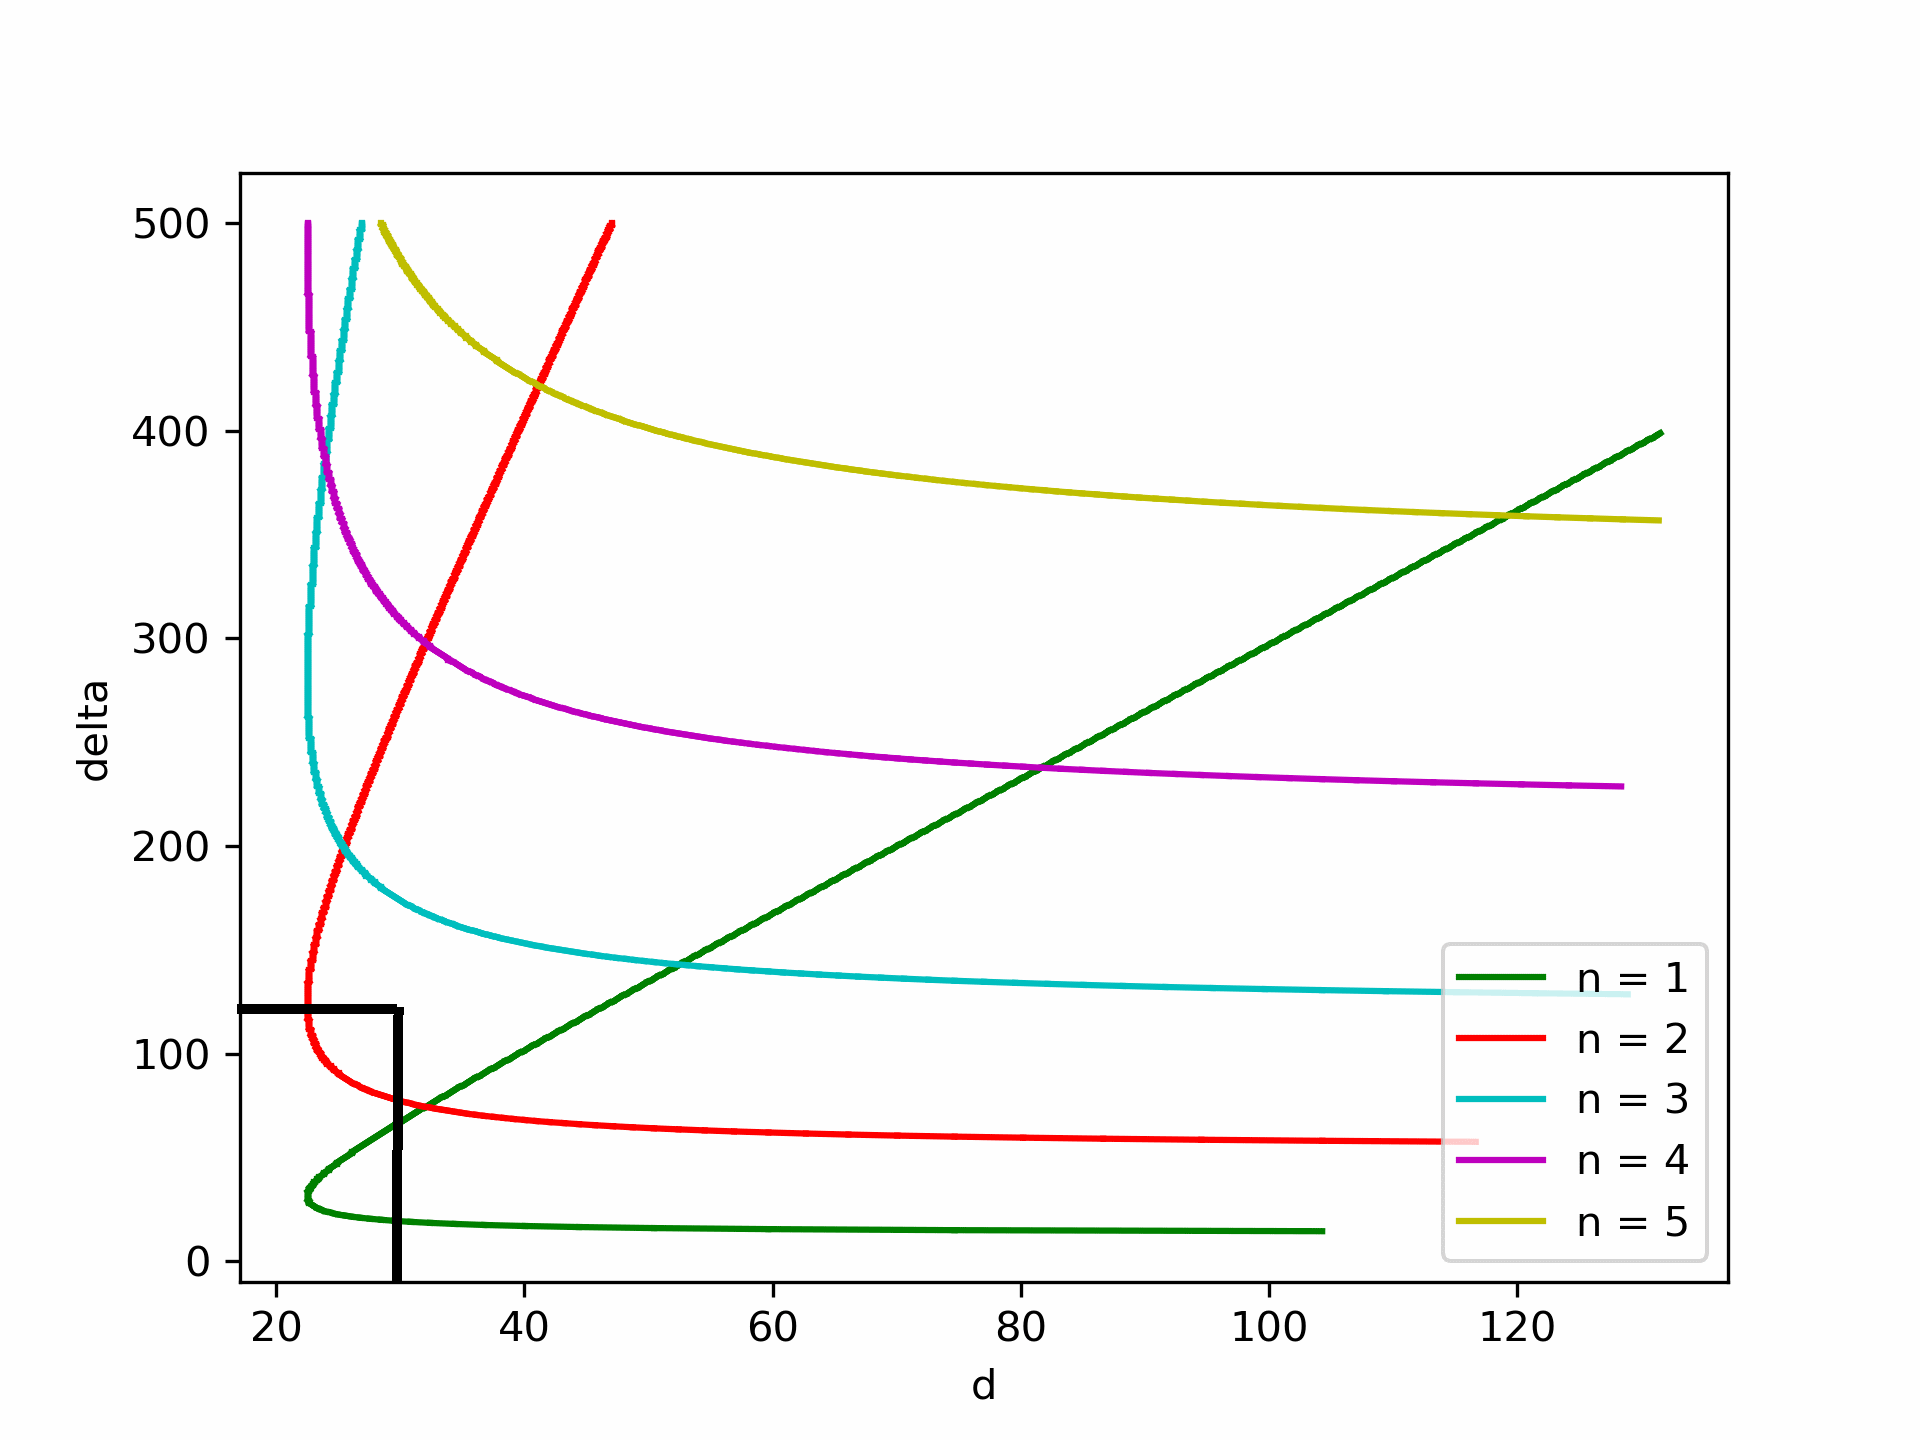
\includegraphics[width=0.4\textwidth]{diagrammes_turing1.png}
\end{subfigure}
\begin{subfigure}
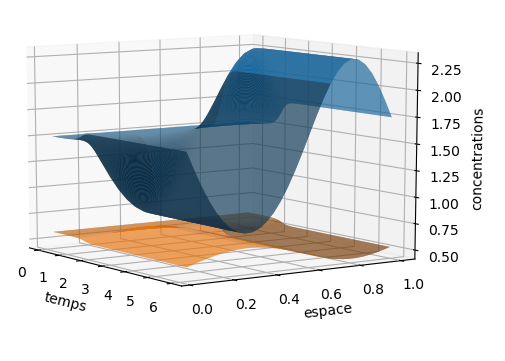
\includegraphics[width=0.4\textwidth]{graph1.png}
\end{subfigure}
\caption{\label{fig:graph1}Instabilité du mode 2}
\end{figure}
\end{frame}


\begin{frame}{Résolution par la méthode d’Euler implicite}
\textbf{Résultats}\\
Prévision : instabilité du mode 4, vérifiée
\begin{figure}
\begin{subfigure}
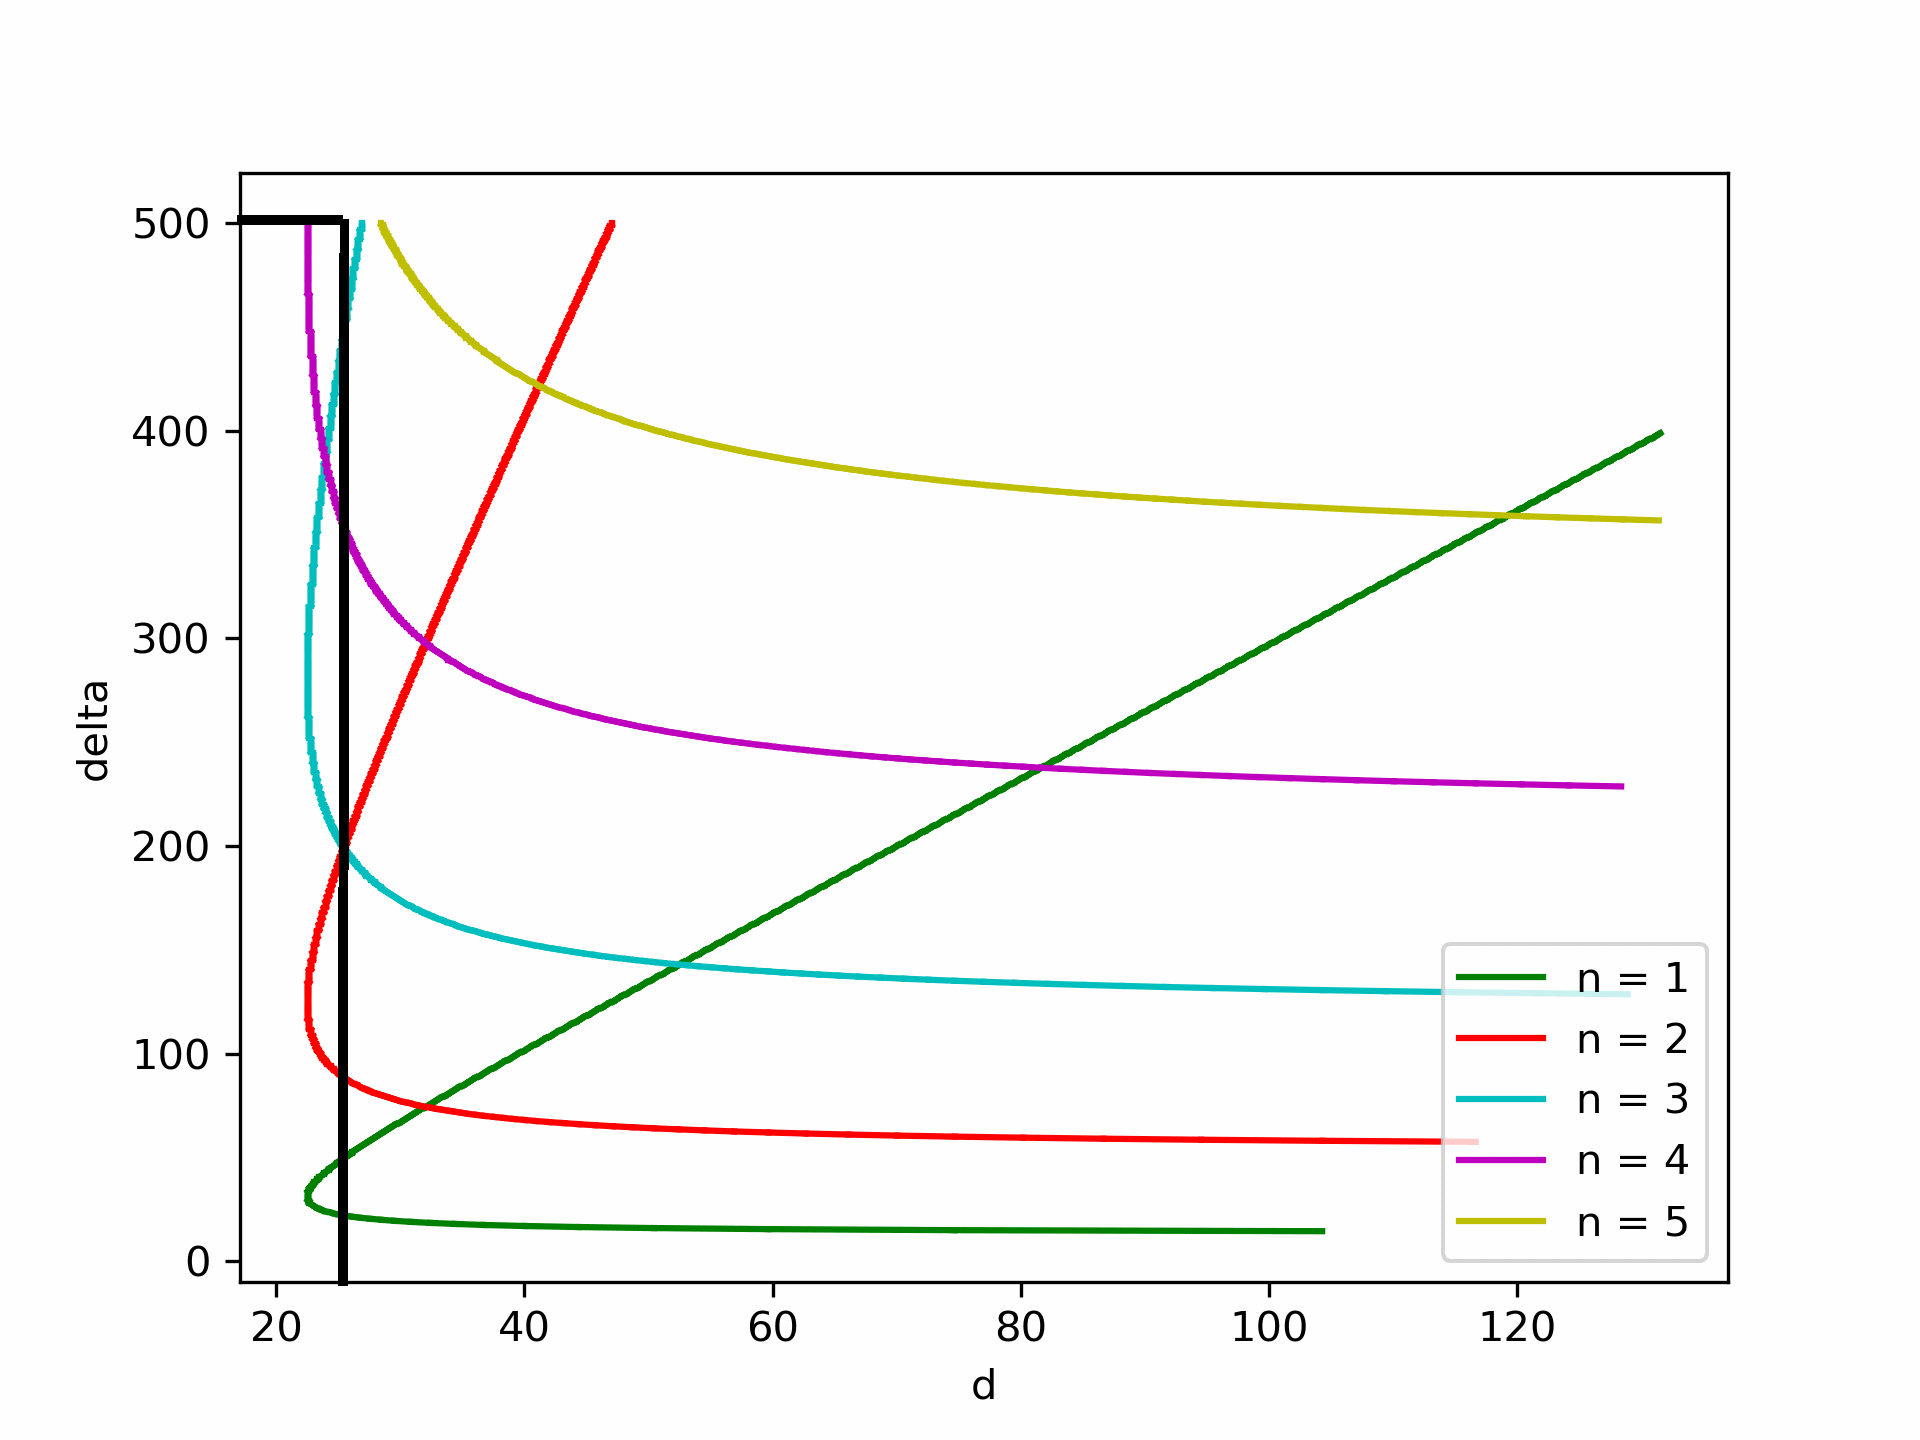
\includegraphics[width=0.4\textwidth]{diagrammes_turing2.png}
\end{subfigure}
\begin{subfigure}
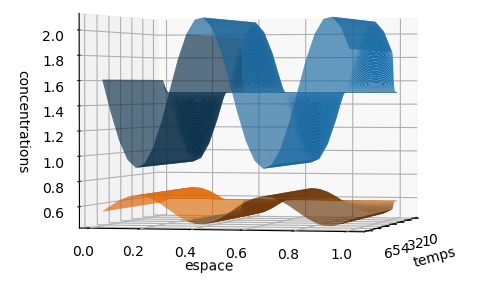
\includegraphics[width=0.4\textwidth]{graph2.png}
\end{subfigure}
\caption{\label{fig:graph1}Instabilité du mode 4}
\end{figure}
\end{frame}

\begin{frame}{Résolution par la méthode d’Euler implicite}
\textbf{Remarques}\\
Superposition de modes instables
\begin{figure}
\begin{subfigure}
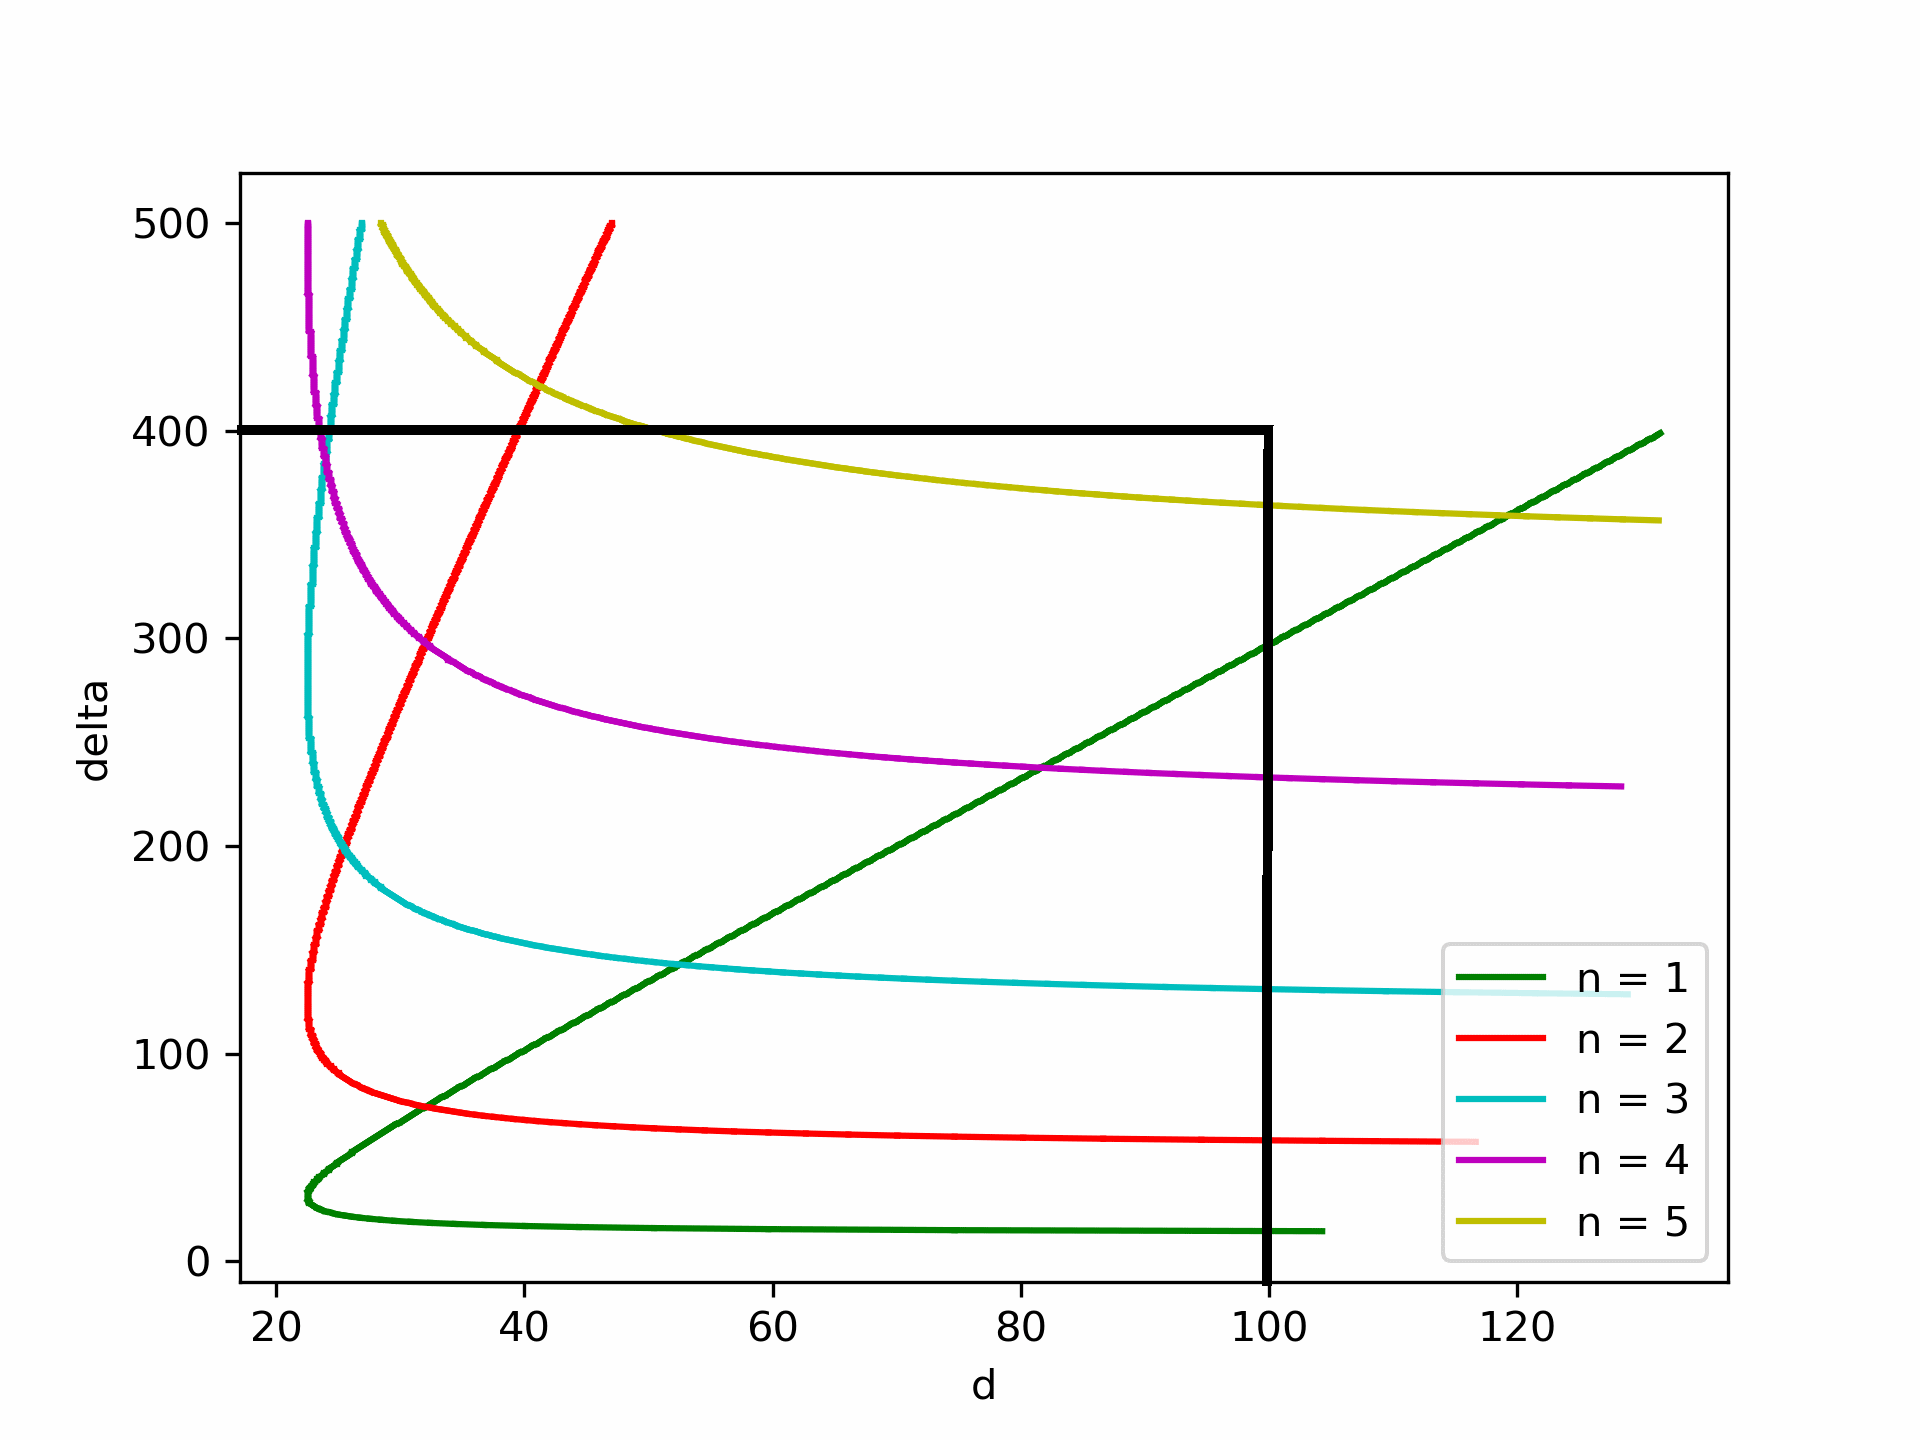
\includegraphics[width=0.4\textwidth]{diagrammes_turing3.png}
\end{subfigure}
\begin{subfigure}
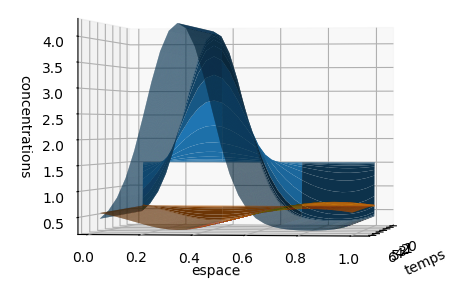
\includegraphics[width=0.4\textwidth]{graph3.png}
\end{subfigure}
\caption{\label{fig:graph3}Superposition des modes instables}
\end{figure}
\end{frame}


\begin{frame}{Résolution par la méthode d’Euler implicite}
\textbf{Remarques}\\
Plus on est proche de $d_{critique}$, plus la convergence apparaît tardivement : 
\begin{figure}
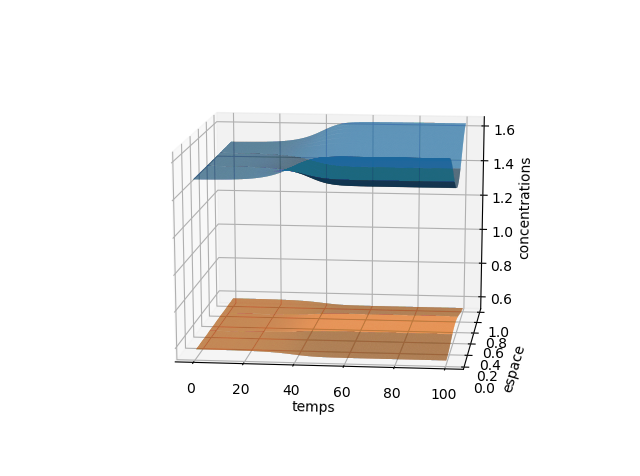
\includegraphics[width=0.4\textwidth]{graph4.png}
\caption{\label{fig:graph4} $d = 23.1$, convergence après 50 secondes}
\end{figure}
\end{frame}

\end{document}
